% Préambule commun des schémas TikZ (compilés séparément par construire_figures.py)
\documentclass[tikz,border=3pt]{standalone}
\usepackage[T1]{fontenc}
\usepackage[utf8]{inputenc}
\usepackage{lmodern}
\usepackage{amsmath,amssymb}
\usepackage{bm}
\usepackage[american,siunitx,straightvoltages]{circuitikz}
\usetikzlibrary{arrows.meta,positioning,calc,decorations.pathmorphing,
  decorations.markings,decorations.pathreplacing,patterns,shapes.geometric,
  shapes.misc,shapes.multipart,fit,backgrounds,3d,intersections,matrix}

\ctikzset{bipoles/length=1.1cm, amplifiers/scale=0.85, tripoles/op amp/width=1.4}

\tikzset{
  >={Latex[length=2mm,width=1.4mm]},
  every picture/.style={line width=0.6pt, font=\small},
  % schémas-blocs
  bloc/.style={draw, minimum width=1.5cm, minimum height=0.9cm, align=center,
               inner sep=3pt, fill=white},
  somme/.style={draw, circle, minimum size=4.5mm, inner sep=0pt, fill=white,
                path picture={\draw (path picture bounding box.north west)
                  -- (path picture bounding box.south east)
                  (path picture bounding box.north east)
                  -- (path picture bounding box.south west);}},
  gain/.style={draw, isosceles triangle, isosceles triangle apex angle=60,
               minimum size=8mm, inner sep=1pt, fill=white},
  bruit/.style={draw, circle, minimum size=4.5mm, inner sep=0pt, fill=white,
                path picture={\node at (path picture bounding box.center)
                  {\scriptsize$\ast$};}},
  cadre/.style={draw, dashed, rounded corners=1pt},
  cadrept/.style={draw, dash dot, rounded corners=1pt},
  fleche/.style={->},
  % mécanique
  bati/.style={pattern=north east lines, draw=none},
  ressort/.style={decorate, decoration={coil, aspect=0.4, segment length=2.2mm,
                  amplitude=2mm, pre length=2mm, post length=2mm}},
  zigzag/.style={decorate, decoration={zigzag, segment length=2mm,
                  amplitude=1.6mm, pre length=2mm, post length=2mm}},
  pivot/.style={draw, circle, fill=white, minimum size=2.2mm, inner sep=0pt},
  masse/.style={draw, fill=gray!25, minimum width=1.4cm, minimum height=0.8cm},
  cote/.style={<->, line width=0.4pt},
  axe/.style={->, line width=0.6pt},
  trait mixte/.style={dash dot, line width=0.4pt},
}

% Encastrement / bâti hachuré : \bati{(x1,y1)}{(x2,y2)} trace une ligne et ses hachures dessous
\newcommand{\bati}[3][0.18]{%
  \fill[pattern=north east lines] #2 rectangle ($#3+(0,-#1)$);
  \draw[line width=0.8pt] #2 -- #3;}

% Transducteur (deux cercles entrelacés) : \pic (t) at (x,y) {transducteur};  -> (t-o) entrée, (t-e) sortie
\tikzset{
  transducteur/.pic={\draw (-0.13,0) circle (0.24); \draw (0.13,0) circle (0.24);
    \coordinate (-o) at (-0.37,0); \coordinate (-e) at (0.37,0);
    \coordinate (-n) at (0,0.24); \coordinate (-s) at (0,-0.24);},
  bobine/.style={decorate, decoration={coil, aspect=0.7, segment length=1.4mm,
                 amplitude=1.6mm, pre length=1mm, post length=1mm}},
  sourcebruit/.style={draw, circle, minimum size=5mm, inner sep=0pt, fill=white,
                 label={[inner sep=0pt]center:$\ast$}},
  sourcecourant/.style={draw, circle, minimum size=5mm, inner sep=0pt, fill=white,
                 label={[inner sep=0pt]center:$\circledast$}},
}

% Composants compacts (pour les petits boîtiers des schémas-blocs)
\newcommand{\resistance}[2]{% de #1 à #2 (quelconque)
  \draw #1 -- ($#1!0.22!#2$) ($#1!0.78!#2$) -- #2;
  \draw[decorate, decoration={zigzag, segment length=1.5mm, amplitude=1.1mm}]
    ($#1!0.22!#2$) -- ($#1!0.78!#2$);}
\newcommand{\condensateur}[2]{% horizontal de #1 à #2
  \draw #1 -- ($($#1!0.5!#2$)+(-0.05,0)$) ($($#1!0.5!#2$)+(0.05,0)$) -- #2;
  \draw[line width=1pt] ($($#1!0.5!#2$)+(-0.05,0.14)$) -- ($($#1!0.5!#2$)+(-0.05,-0.14)$)
                        ($($#1!0.5!#2$)+(0.05,0.14)$) -- ($($#1!0.5!#2$)+(0.05,-0.14)$);}
% R // C horizontal : \RparC{(x,y)}{longueur}{écart}  (centre, longueur totale, écart vertical)
\newcommand{\RparC}[3]{%
  \coordinate (rcA) at ($#1+(-#2/2,0)$); \coordinate (rcB) at ($#1+(#2/2,0)$);
  \draw (rcA) -- ++(0.15,0) coordinate (rcA1) (rcB) -- ++(-0.15,0) coordinate (rcB1);
  \draw (rcA1) -- ++(0,#3/2) (rcA1) -- ++(0,-#3/2) (rcB1) -- ++(0,#3/2) (rcB1) -- ++(0,-#3/2);
  \resistance{($(rcA1)+(0,#3/2)$)}{($(rcB1)+(0,#3/2)$)}
  \condensateur{($(rcA1)+(0,-#3/2)$)}{($(rcB1)+(0,-#3/2)$)}}

\newcommand{\porte}[1]{% porte analogique (2 inverseurs) centrée en #1
  \draw ($#1+(-0.75,-0.6)$) rectangle ($#1+(0.75,0.6)$);
  \foreach \dy in {0.28,-0.28} {
    \fill ($#1+(-0.25,\dy)$) circle (1pt) ($#1+(0.3,\dy+0.12)$) circle (1pt) ($#1+(0.3,\dy-0.12)$) circle (1pt);
    \draw ($#1+(-0.25,\dy)$) -- ($#1+(0.3,\dy+0.12)$);}}
\begin{document}
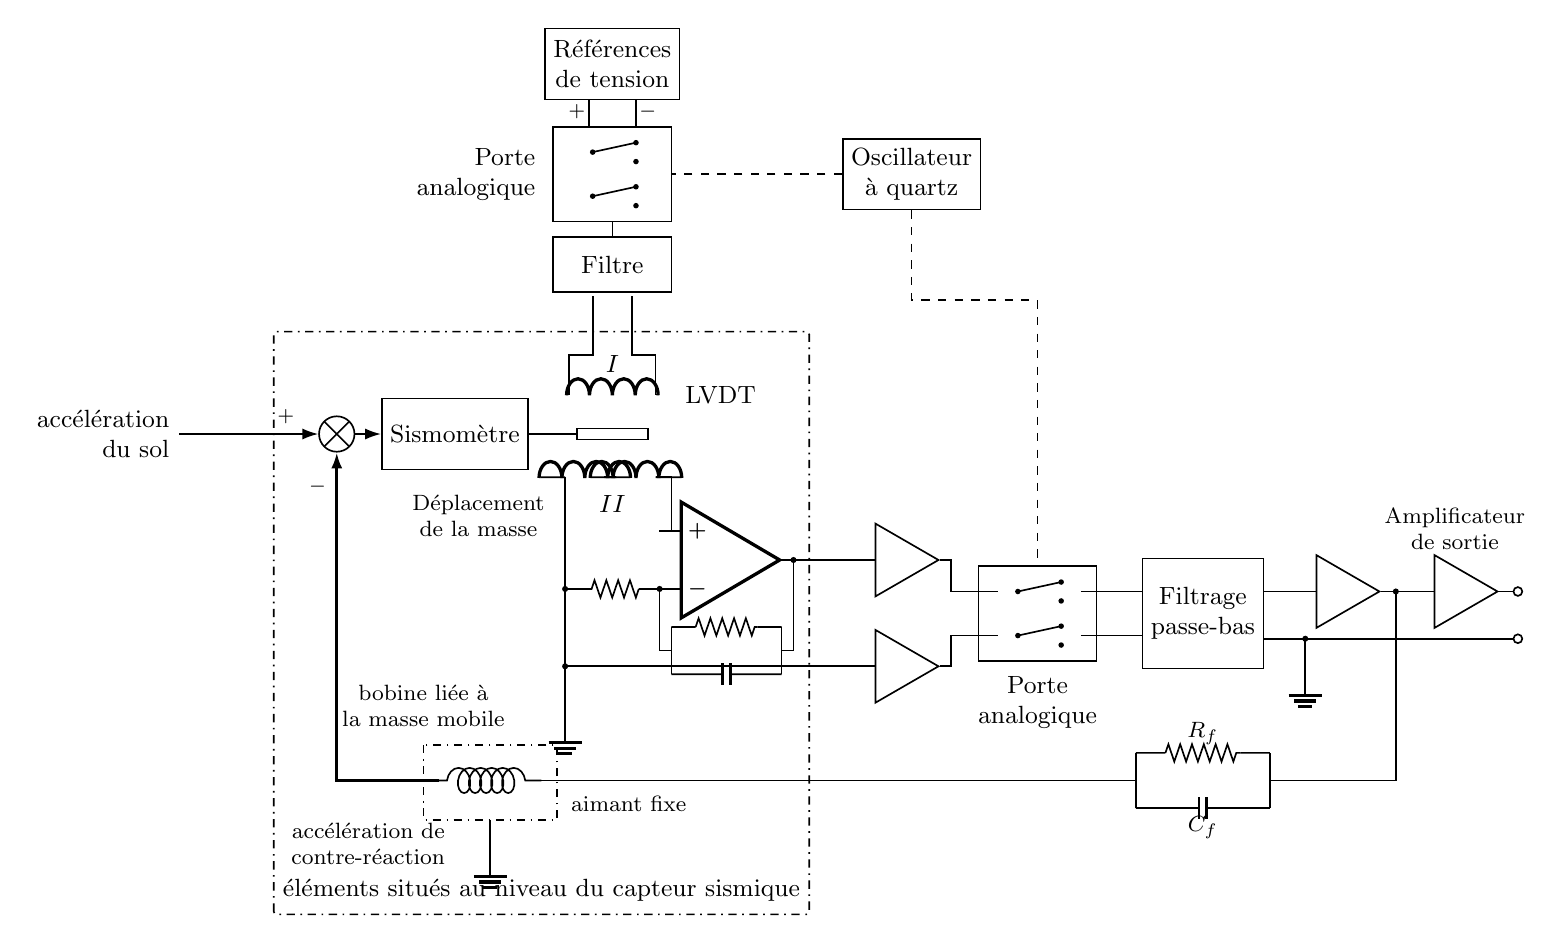
\begin{tikzpicture}[font=\small]
  % ---------- excitation ----------
  \node[bloc, align=center] (ref) at (5.0,7.3) {Références\\de tension};
  \porte{(5.0,5.9)} \node[left, align=right] at (4.15,5.9) {Porte\\analogique};
  \draw (4.7,6.85) -- (4.7,6.5) (5.3,6.85) -- (5.3,6.5);
  \node[font=\scriptsize] at (4.55,6.7) {$+$}; \node[font=\scriptsize] at (5.45,6.7) {$-$};
  \node[bloc, minimum height=7mm] (fil) at (5.0,4.75) {Filtre};
  \draw (5.0,5.3) -- (fil.north);
  \node[bloc, align=center] (osc) at (8.8,5.9) {Oscillateur\\à quartz};
  \draw[dashed] (osc.west) -- (5.75,5.9);
  % ---------- éléments au niveau du capteur ----------
  \draw[cadrept] (0.7,-3.5) rectangle (7.5,3.9);
  \node at (4.1,-3.2) {éléments situés au niveau du capteur sismique};
  \node[somme] (s) at (1.5,2.6) {};
  \node[bloc] (sis) at (3.0,2.6) {Sismomètre};
  \draw[->] (-0.5,2.6) node[left, align=right] {accélération\\du sol} -- (s) node[above left, pos=0.9] {\scriptsize$+$};
  \draw[->] (s) -- (sis);
  % LVDT
  \draw[fill=white] (4.55,2.53) rectangle (5.45,2.67);
  \draw (sis.east) -- (4.55,2.6);
  \draw (4.45,3.1) to[L] (5.55,3.1);
  \draw (4.75,4.35) -- (4.75,3.6) -| (4.45,3.1);
  \draw (5.25,4.35) -- (5.25,3.6) -| (5.55,3.1);
  \node[above] at (5.0,3.25) {$I$};
  \draw (4.4,2.05) to[L] (4.9,2.05); \draw (5.05,2.05) to[L] (5.55,2.05);
  \draw (4.9,2.05) -- (5.05,2.05);
  \node[below] at (5.0,1.95) {$II$};
  \node[right] at (5.8,3.1) {LVDT};
  \node[below, align=center, font=\footnotesize] at (3.3,1.95) {Déplacement\\de la masse};
  % amplificateur de tête
  \draw (6.5,1.0) node[op amp, noinv input up, scale=0.75] (tete) {};
  \draw (5.55,2.05) -- (5.75,2.05) |- (tete.+);
  \draw (4.4,2.05) -- (4.4,-0.9) node[ground] {};
  \draw (tete.-) -- (5.6,0.82 |- tete.-) coordinate (fb);
  \fill (fb) circle (1.1pt) (4.4,0 |- fb) circle (1.1pt);
  \resistance{(fb)}{(4.4,0 |- fb)}
  \draw (fb) -- (5.6,-0.15);
  \RparC{(6.45,-0.15)}{1.7}{0.6}
  \draw (7.3,-0.15) -- (7.3,0 |- tete.out);
  \fill (7.3,0 |- tete.out) circle (1.1pt);
  % bobine de contre-réaction
  \draw[dash dot] (2.6,-1.35) rectangle (4.3,-2.3);
  \draw[bobine] (2.8,-1.8) -- (4.1,-1.8);
  \node[align=center, font=\footnotesize] at (2.6,-0.85) {bobine liée à\\la masse mobile};
  \node[font=\footnotesize, right] at (4.35,-2.1) {aimant fixe};
  \draw[->, line width=1pt] (2.8,-1.8) -- (1.5,-1.8) -- (s.south) node[below left, pos=0.95] {\scriptsize$-$};
  \node[align=center, font=\footnotesize] at (1.9,-2.6) {accélération de\\contre-réaction};
  \draw (3.45,-2.3) -- (3.45,-2.6) node[ground] {};
  % ---------- démodulation et sortie ----------
  \node[gain] (b1) at (8.6,1.0) {};
  \node[gain] (b2) at (8.6,-0.35) {};
  \draw (tete.out) -- (b1.west);
  \draw (4.4,-0.35) -- (b2.west); \fill (4.4,-0.35) circle (1.1pt);
  \porte{(10.4,0.32)} \node[below, align=center] at (10.4,-0.35) {Porte\\analogique};
  \draw (b1.east) -- (9.3,1.0) |- (9.9,0.6); \draw (b2.east) -- (9.3,-0.35) |- (9.9,0.04);
  \draw[dashed] (osc.south) -- (8.8,4.3) -| (10.4,0.92);
  \node[bloc, align=center, minimum height=1.4cm] (pb) at (12.5,0.32) {Filtrage\\passe-bas};
  \draw (10.95,0.6) -- (pb.west |- 0,0.6) (10.95,0.04) -- (pb.west |- 0,0.04);
  \node[gain] (g) at (14.2,0.6) {};
  \draw (pb.east |- 0,0.6) -- (g.west);
  \node[gain] (gs) at (15.7,0.6) {};
  \draw (g.east) -- (gs.west); \draw (gs.east) -- (16.5,0.6) node[ocirc] {};
  \draw (pb.east |- 0,0.0) -- (16.5,0.0) node[ocirc] {};
  \fill (13.8,0.0) circle (1.1pt); \draw (13.8,0.0) -- (13.8,-0.3) node[ground] {};
  \node[above, align=center, font=\footnotesize] at (15.7,1.0) {Amplificateur\\de sortie};
  % contre-réaction R_f // C_f
  \fill (14.95,0.6) circle (1.1pt);
  \draw (14.95,0.6) -- (14.95,-1.8) -- (13.5,-1.8);
  \RparC{(12.5,-1.8)}{2.0}{0.7}
  \node[font=\footnotesize] at (12.5,-1.2) {$R_f$}; \node[font=\footnotesize] at (12.5,-2.4) {$C_f$};
  \draw (11.5,-1.8) -- (4.1,-1.8);
\end{tikzpicture}
\end{document}
